% ================================================================
% The Retrieve and Connect version of latex/starters/retrieval/KS3/negativesPowersBidmasStarters_workedSolutions.tex
%
% This is the same deck as the one above, made by renaming the titles in it.
% Every slide that was a numbered starter is now titled
% "Retrieve and Connect", and the word is renamed wherever else a title
% used it. Nothing outside a title has been changed.
%
%   made from           latex/starters/retrieval/KS3/negativesPowersBidmasStarters_workedSolutions.tex
%   retitling rules     version 1
%
% Please don't edit this file. It is written again from the one it was
% made from whenever that changes, so an edit here would be lost - edit
% that file instead and this one follows.
% ================================================================
% Root file used ashow macros
\documentclass{beamer}
\usepackage{tikz}
\usetikzlibrary{calc, arrows.meta}
\usepackage{xcolor}
\usepackage{multicol}
\usepackage{amsmath}
\usepackage{amssymb}

% ================================================================
% Retrieval starters for a Year 7 top set, used across the negative
% numbers, powers and roots, and BIDMAS units.
%
% The class has already covered inequalities, rounding, written methods
% for adding and subtracting decimals (with money problems), and written
% methods for multiplying and dividing, including place value and
% multiplying and dividing by powers of 10. Each starter uses more of the
% new units than the one before:
%
%   1  ordering and comparing negative numbers, on number lines
%   2  adding and subtracting across zero
%   3  adding and subtracting negative numbers
%   4  multiplying and dividing negative numbers
%   5  squares, cubes, square roots and cube roots
%   6  index notation, powers of 10, and estimating square roots
%   7  BIDMAS
%   8  BIDMAS with powers, roots and negative numbers
%
% The methods follow the ones the class was taught:
%   - A scaffolded decimal multiplication is scaffolded for both methods,
%     the lattice method and scaling to whole numbers (make both numbers
%     whole, multiply, then divide by the power of 10 used). The scaling
%     scaffold sits under the lattice with "or" between them, so that
%     pupils can see they only need to do one of the two.
%   - Division by a decimal is done with equivalent fractions: the
%     division is written as a fraction, and the numerator and denominator
%     are multiplied by the same power of 10.
%   - Bus stop division turns a division or a fraction into a decimal that
%     either stops (7 / 8 in starter 1) or recurs (2 / 3 in starter 2, and
%     then without a diagram in starters 3, 4, 7 and 8).
%   - Dividing and writing a fraction are shown to be the same thing,
%     using baguettes shared between teachers (starters 3 and 6), and the
%     fraction bar is treated as a division in BIDMAS (starters 7 and 8).
% The scaffolds fade: starter 4 gives the lattice's decimal points and a
% full equivalent-fraction chain, starter 5 leaves the decimal points for
% pupils to mark, and starter 6 leaves more of the chain out. The bus stop
% divisions are drawn out for pupils in starters 1 and 2 only.
%
% The last question on each starter is a challenge.
% ================================================================

\setbeamertemplate{navigation symbols}{}
\setbeamersize{text margin left=0.4cm, text margin right=0.4cm}
\setlength{\multicolsep}{2pt}
\setlength{\columnsep}{20pt}

% ================================================================
% Answer-overlay helpers
% ================================================================
\newcommand{\ablank}[1]{%
  \alt<2>{\textcolor{red}{#1}}{\underline{\phantom{#1}}}%
}
\newcommand{\ashow}[1]{\uncover<2->{\textcolor{red}{\small #1}}}
\newcommand{\ashowq}[1]{\alt<2->{\textcolor{red}{\small #1}}{?}}

% Answers drawn straight on to a TikZ diagram, revealed on overlay 2 like \ashow.
% Space is reserved on overlay 1, so the diagram does not move between slides.
\usetikzlibrary{overlay-beamer-styles}
\tikzset{
  ans/.style     = {red, thick, visible on=<2->},
  ansfill/.style = {red!15, visible on=<2->},
  anslab/.style  = {red, font=\tiny, visible on=<2->},
}

% Used by the worked solutions rather than by this deck, so that each worked
% solution is first a question with room to write in and then the answer.
\newlength{\aworkpad}
\setlength{\aworkpad}{8mm}
\newcommand{\awork}[1]{%
  \par\vspace{\aworkpad}%
  \uncover<2->{#1}%
  \par\vspace{\aworkpad}%
}

% Every question list on these slides is tight, so that the diagram column and
% the question column both finish inside the slide.
\newcommand{\tightlist}{%
  \setlength{\itemsep}{0pt}\setlength{\parskip}{0pt}\setlength{\topsep}{0pt}%
}

% A pattern of calculations set out in a column under a diagram, with the
% equals signs lined up: \begin{pattern} 5-2 & 3\\ ... \end{pattern}
\newenvironment{pattern}[1]
  {\par\vspace{0.5em}{\scriptsize\bfseries #1}\par\vspace{0.2em}\footnotesize
   \hspace*{0.3cm}\begin{tabular}{@{}r@{${}={}$}l@{}}}
  {\end{tabular}\par}

% The two methods for a decimal multiplication are set one above the other
% in the diagram column, the lattice first and then the scaling scaffold, with
% \orrule between them to show that pupils only need to do one of the two.
\newcommand{\orrule}{%
  \par\vspace{0.2em}\noindent
  \tikz[baseline=-0.6ex]{\draw[gray] (0,0) -- (1.55,0);
    \node[font=\footnotesize\bfseries] at (1.95,0) {or};
    \draw[gray] (2.35,0) -- (3.9,0);}%
  \par\vspace{0.1em}}
\newenvironment{scaling}
  {\par{\scriptsize\bfseries Scaling to whole numbers}\par\vspace{0.15em}\footnotesize
   \hspace*{0.15cm}\begin{tabular}{@{}l@{}}}
  {\end{tabular}\par}

% A temperature in degrees Celsius: \dC{-4}.
\newcommand{\dC}[1]{$#1\,^{\circ}$C}

% ================================================================
% The pictures these starters are built from.
%
% Every number line is about 3.8 cm long and starts at x = 0. Each is drawn
% in a scope whose x unit is one step along that line, shifted so that its
% left end is at 0; a coordinate on the line is then the value it stands for.
% ================================================================
\tikzset{
  dhead/.style = {font=\scriptsize\bfseries, anchor=west},
  nlab/.style  = {font=\scriptsize, below, inner sep=2pt},
  vans/.style  = {anslab, font=\scriptsize},
}

% ---- Lattice multiplication, drawn as on the lattice method slides ----
% The top-left corner of the lattice is at the origin and each cell is one
% unit, so a lattice is drawn inside a scope that sets the cell size. The
% digits of the first number go along the top and the digits of the second
% number down the right-hand side. Each cell is cut by a diagonal from its
% top-right corner to its bottom-left corner, with the tens digit of its
% product above the diagonal and the units digit below it. The digits of the
% answer are read down the left-hand side and then along the bottom.
\tikzset{
  lcellline/.style = {draw=blue!55!black, line width=0.6pt},
  ldiagline/.style = {draw=blue!55!black!45, line width=0.5pt},
  ldigit/.style    = {font=\scriptsize\bfseries},
}
% \lgrid{cols}{rows}: the cells and their diagonals
\newcommand{\lgrid}[2]{%
  \foreach \c in {1,...,#1}{%
    \foreach \r in {1,...,#2}{%
      \draw[lcellline] ({\c-1},{-\r+1}) rectangle ({\c},{-\r});
      \draw[ldiagline] ({\c},{-\r+1}) -- ({\c-1},{-\r});}}%
}
% \ltop{col}{digit} and \lside{cols}{row}{digit}: the two numbers
\newcommand{\ltop}[2]{\node[ldigit] at ({#1-0.5},0.3) {#2};}
\newcommand{\lside}[3]{\node[ldigit] at ({#1+0.3},{-#2+0.5}) {#3};}
% Answers. \lcell{col}{row}{tens}{units} fills a cell; \lleft{row}{digit} and
% \lbot{rows}{col}{digit} are the digits of the answer.
\newcommand{\lcell}[4]{%
  \node[vans] at ({#1-0.7},{-#2+0.7}) {#3};
  \node[vans] at ({#1-0.3},{-#2+0.3}) {#4};}
\newcommand{\lleft}[2]{\node[vans, font=\scriptsize\bfseries] at (-0.3,{-#1+0.5}) {#2};}
\newcommand{\lbot}[3]{\node[vans, font=\scriptsize\bfseries] at ({#2-0.5},{-#1-0.3}) {#3};}
% A decimal point on the edge of a lattice, or in its answer.
\newcommand{\lpoint}[3][]{\fill[#1] (#2,#3) circle (1.7pt);}

% ---- Bus stop division ----
% The dividend sits on the baseline y = 0 and the answer on y = 0.55, digit
% above digit, with the bus stop drawn between them. A remainder carried to
% the next digit is written small, just before that digit. \busframe{divisor}
% {right end} draws the divisor and the bus stop.
\tikzset{
  bsd/.style     = {font=\footnotesize, inner sep=0pt, anchor=base},
  bsa/.style     = {bsd, red, visible on=<2->},
  bscarry/.style = {font=\tiny, inner sep=0pt, anchor=base, red, visible on=<2->},
}
\newcommand{\busframe}[2]{%
  \node[bsd, anchor=base east] at (-0.1,0) {$#1$};
  \draw[thick] (0,-0.12) -- (0,0.4) -- (#2,0.4);}

% ---- Baguettes ----
% \baguette{x}{y}: a baguette 3.6 cm long and 0.36 cm high, with its
% bottom-left corner at (x,y) and the usual diagonal scores across its top.
% The scores sit in the middle of each quarter, so they never land on a cut.
\newcommand{\baguette}[2]{%
  \draw[fill=orange!35!yellow!40, draw=brown!70!black, thick, rounded corners=0.17cm]
    (#1,#2) rectangle ++(3.6,0.36);
  \foreach \i in {0,...,3}
    \draw[brown!60!black, line width=0.5pt] ({#1+0.9*\i+0.35},{#2+0.08}) -- ++(0.2,0.2);}
% \bagcuts{y}: the three cuts that split the baguette at height y into quarters
\newcommand{\bagcuts}[1]{%
  \foreach \i in {1,2,3} \draw[ans] ({0.9*\i},{#1-0.06}) -- ({0.9*\i},{#1+0.42});}
% \baglabels{y}{a}{b}{c}{d}: who gets each quarter, written under it
\newcommand{\baglabels}[5]{%
  \foreach \i/\lab in {0/#2, 1/#3, 2/#4, 3/#5}
    \node[vans, inner sep=1pt] at ({0.9*\i+0.45},{#1-0.16}) {\lab};}

\title{Negative Numbers, Powers \& BIDMAS: Retrieve and Connects}
\author{}
\date{}

\begin{document}

\frame{\titlepage}

\begin{frame}{Contents}
\small
\begin{columns}[T]
\begin{column}{0.5\textwidth}
\textbf{Questions and short answers}
\begin{itemize}
\item \hyperlink{q-st1}{\beamergotobutton{Retrieve and Connect 1}}
\item \hyperlink{q-st2}{\beamergotobutton{Retrieve and Connect 2}}
\item \hyperlink{q-st3}{\beamergotobutton{Retrieve and Connect 3}}
\item \hyperlink{q-st4}{\beamergotobutton{Retrieve and Connect 4}}
\item \hyperlink{q-st5}{\beamergotobutton{Retrieve and Connect 5}}
\item \hyperlink{q-st6}{\beamergotobutton{Retrieve and Connect 6}}
\item \hyperlink{q-st7}{\beamergotobutton{Retrieve and Connect 7}}
\item \hyperlink{q-st8}{\beamergotobutton{Retrieve and Connect 8}}
\end{itemize}
\end{column}
\begin{column}{0.5\textwidth}
\textbf{Worked solutions}
\begin{itemize}
\item \hyperlink{work-st1}{\beamergotobutton{Retrieve and Connect 1}}
\item \hyperlink{work-st2}{\beamergotobutton{Retrieve and Connect 2}}
\item \hyperlink{work-st3}{\beamergotobutton{Retrieve and Connect 3}}
\item \hyperlink{work-st4}{\beamergotobutton{Retrieve and Connect 4}}
\item \hyperlink{work-st5}{\beamergotobutton{Retrieve and Connect 5}}
\item \hyperlink{work-st6}{\beamergotobutton{Retrieve and Connect 6}}
\item \hyperlink{work-st7}{\beamergotobutton{Retrieve and Connect 7}}
\item \hyperlink{work-st8}{\beamergotobutton{Retrieve and Connect 8}}
\end{itemize}
\end{column}
\end{columns}
\end{frame}

%------------------------------------------------------------------
% STARTER 1: Ordering and comparing negative numbers
%------------------------------------------------------------------
\begin{frame}[t]{Retrieve and Connect: Ordering Negative Numbers}
\hypertarget{q-st1}{}
\begin{columns}[T,onlytextwidth]

\column{0.36\textwidth}
\vspace{-0.4em}
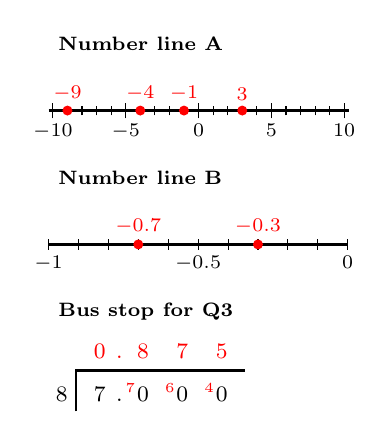
\begin{tikzpicture}[every node/.style={font=\scriptsize}]

% ---- Number line A: -10 to 10 ----
\begin{scope}[x=0.185cm, shift={(10.3,0)}]
\node[dhead] at (-10.3,0.85) {Number line A};
\draw[thick] (-10.3,0) -- (10.3,0);
\foreach \v in {-10,...,10} \draw (\v,-0.06) -- (\v,0.06);
\foreach \v in {-10,-5,0,5,10} {
  \draw (\v,-0.1) -- (\v,0.1);
  \node[nlab] at (\v,-0.1) {$\v$};
}
% --- Q4 answer: the four temperatures ---
\foreach \v in {-9,-4,-1,3} {
  \fill[ans] (\v,0) circle (1.8pt);
  \node[vans, above, inner sep=1.5pt] at (\v,0.07) {$\v$};
}
\end{scope}

% ---- Number line B: -1 to 0 in tenths ----
\begin{scope}[x=3.8cm, shift={(1,0)}, yshift=-1.7cm]
\node[dhead] at (-1,0.85) {Number line B};
\draw[thick] (-1,0) -- (0,0);
\foreach \v in {-1,-0.9,...,0.01} \draw (\v,-0.07) -- (\v,0.07);
\foreach \v in {-1,-0.5,0} \node[nlab] at (\v,-0.07) {$\v$};
% --- Q9 answer: -0.7 and -0.3 ---
\foreach \v in {-0.7,-0.3} {
  \fill[ans] (\v,0) circle (1.8pt);
  \node[vans, above, inner sep=1.5pt] at (\v,0.07) {$\v$};
}
\end{scope}

% ---- Bus stop division for 7 / 8, with the zeros written in ----
\begin{scope}[xshift=0.35cm, yshift=-3.7cm]
\node[dhead] at (-0.35,1.15) {Bus stop for Q3};
\busframe{8}{2.15}
\foreach \x/\d in {0.3/7, 0.55/., 0.85/0, 1.35/0, 1.85/0} \node[bsd] at (\x,0) {$\d$};
% --- Q3 answer: 7 / 8 = 0.875, carrying 7, then 6, then 4 ---
\foreach \x/\d in {0.3/0, 0.55/., 0.85/8, 1.35/7, 1.85/5} \node[bsa] at (\x,0.55) {$\d$};
\foreach \x/\c in {0.85/7, 1.35/6, 1.85/4} \node[bscarry] at ({\x-0.16},0.12) {$\c$};
\end{scope}

\end{tikzpicture}

\column{0.64\textwidth}
\vspace{-1.5em}
\footnotesize
\begin{enumerate}\tightlist
\begin{multicols}{2}
  \item $3.8\times100$ \ashow{$=380$}
  \columnbreak
  \item $45\div1000$ \ashow{$=0.045$}
\end{multicols}
  \item Complete the bus stop division to write $\frac78$ as a decimal.
        \ashow{$0.875$}
  \item At midday it is \dC{-4} in Oslo, \dC{-9} in Moscow, \dC{3} in London and
        \dC{-1} in Reykjavík. Mark these on number line A. Write them in order,
        coldest first.
        \ashow{$-9$, \; $-4$, \; $-1$, \; $3$}
  \item[] Write $<$ or $>$ in each box.
{\setlength{\columnsep}{14pt}%
\begin{multicols}{3}
  \item $-9$ \ablank{$<$} $-4$
  \columnbreak
  \item $-1$ \ablank{$>$} $-10$
  \columnbreak
  \item $0$ \ablank{$>$} $-0.5$
\end{multicols}}
  \item How many degrees warmer is London than Moscow?
        \ashow{$12$ degrees}
  \item Mark $-0.3$ and $-0.7$ on number line B. Which is greater?
        \ashow{$-0.3$, because it is further right}
\begin{multicols}{2}
  \item Round $-4.7$ to the nearest integer.
        \ashow{$-5$}
  \columnbreak
  \item Round $-1.46$ to $1$ decimal place.
        \ashow{$-1.5$}
\end{multicols}
  \item (Challenge) List the integers $n$ with $-3<n\leq1$.
        \ashow{$-2,\ -1,\ 0,\ 1$}
\end{enumerate}
\end{columns}
\end{frame}

\begin{frame}[t]{Worked Solution: Retrieve and Connect 1, Question 1}
\hypertarget{work-st1}{}
\textbf{Question:} $3.8\times100$ \\
\awork{Solution: $3.8 \times 100 = 380$. \\
Multiplying by $100$ shifts the digits two places to the left.}
\end{frame}

\begin{frame}[t]{Worked Solution: Retrieve and Connect 1, Question 2}
\textbf{Question:} $45\div1000$ \\
\awork{Solution: $45 \div 1000 = 0.045$. \\
Dividing by $1000$ shifts the digits three places to the right.}
\end{frame}

\begin{frame}[t]{Worked Solution: Retrieve and Connect 1, Question 3}
\textbf{Question:} Complete the bus stop division to write $\frac78$ as a decimal. \\
\awork{Solution: $7 \div 8 = 0.875$. \\
Bus stop: $8$ into $7$ goes $0$ remainder $7$; $8$ into $70$ goes $8$ remainder $6$; $8$ into $60$ goes $7$ remainder $4$; $8$ into $40$ goes $5$ remainder $0$.}
\end{frame}

\begin{frame}[t]{Worked Solution: Retrieve and Connect 1, Question 4}
\textbf{Question:} At midday it is $-4^\circ$C in Oslo, $-9^\circ$C in Moscow, $3^\circ$C in London and $-1^\circ$C in Reykjavík. Write them in order, coldest first. \\
\awork{Solution: Coldest is furthest left on the number line. \\
Order: $-9^\circ$C, $-4^\circ$C, $-1^\circ$C, $3^\circ$C.}
\end{frame}

\begin{frame}[t]{Worked Solution: Retrieve and Connect 1, Question 5}
\textbf{Question:} Write $<$ or $>$: $-9 \Box -4$. \\
\awork{Solution: $-9 < -4$. \\
$-9$ is further left than $-4$ on the number line, so it is smaller.}
\end{frame}

\begin{frame}[t]{Worked Solution: Retrieve and Connect 1, Question 6}
\textbf{Question:} Write $<$ or $>$: $-1 \Box -10$. \\
\awork{Solution: $-1 > -10$. \\
$-1$ is further right than $-10$, so it is greater.}
\end{frame}

\begin{frame}[t]{Worked Solution: Retrieve and Connect 1, Question 7}
\textbf{Question:} Write $<$ or $>$: $0 \Box -0.5$. \\
\awork{Solution: $0 > -0.5$. \\
$0$ is greater than any negative number.}
\end{frame}

\begin{frame}[t]{Worked Solution: Retrieve and Connect 1, Question 8}
\textbf{Question:} How many degrees warmer is London than Moscow? \\
\awork{Solution: London is $3^\circ$C, Moscow is $-9^\circ$C. \\
Difference $= 3 - (-9) = 3 + 9 = 12$ degrees.}
\end{frame}

\begin{frame}[t]{Worked Solution: Retrieve and Connect 1, Question 9}
\textbf{Question:} Mark $-0.3$ and $-0.7$ on number line B. Which is greater? \\
\awork{Solution: $-0.3$ is to the right of $-0.7$ on the number line. \\
Therefore $-0.3 > -0.7$, so $-0.3$ is greater.}
\end{frame}

\begin{frame}[t]{Worked Solution: Retrieve and Connect 1, Question 10}
\textbf{Question:} Round $-4.7$ to the nearest integer. \\
\awork{Solution: $-4.7$ is between $-5$ and $-4$. \\
It is closer to $-5$, so rounded to the nearest integer it is $-5$.}
\end{frame}

\begin{frame}[t]{Worked Solution: Retrieve and Connect 1, Question 11}
\textbf{Question:} Round $-1.46$ to $1$ decimal place. \\
\awork{Solution: The first decimal place is $4$. The next digit is $6$, so round up. \\
$-1.46$ rounded to $1$ d.p. is $-1.5$.}
\end{frame}

\begin{frame}[t]{Worked Solution: Retrieve and Connect 1, Question 12}
\textbf{Question:} (Challenge) List the integers $n$ with $-3<n\leq1$. \\
\awork{Solution: We need integers greater than $-3$ and less than or equal to $1$. \\
These are $-2$, $-1$, $0$, $1$.}
\end{frame}

%------------------------------------------------------------------
% STARTER 2: Adding and subtracting across zero
%------------------------------------------------------------------
\begin{frame}[t]{Retrieve and Connect: Adding \& Subtracting Across Zero}
\hypertarget{q-st2}{}
\begin{columns}[T,onlytextwidth]

\column{0.36\textwidth}
\vspace{-0.4em}
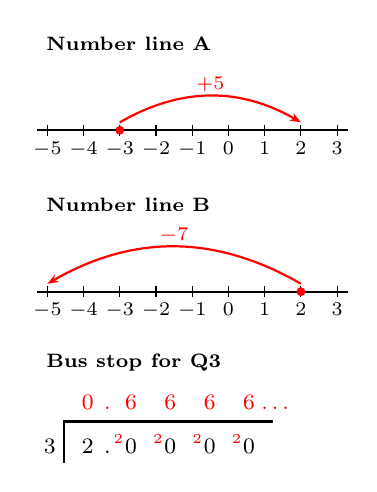
\begin{tikzpicture}[every node/.style={font=\scriptsize}]

% ---- Number line A: -5 to 3, for -3 + 5 ----
\begin{scope}[x=0.46cm, shift={(5.3,0)}]
\node[dhead] at (-5.3,1.1) {Number line A};
\draw[thick] (-5.3,0) -- (3.3,0);
\foreach \v in {-5,...,3} {
  \draw (\v,-0.07) -- (\v,0.07);
  \node[nlab] at (\v,-0.07) {$\v$};
}
% --- Q4 answer: start at -3 and jump 5 to the right ---
\fill[ans] (-3,0) circle (1.6pt);
\draw[ans, -{Stealth[length=4pt]}] (-3,0.1) to[out=30, in=150]
  node[vans, above, inner sep=1pt] {$+5$} (2,0.1);
\end{scope}

% ---- Number line B: -5 to 3, for 2 - 7 ----
\begin{scope}[x=0.46cm, shift={(5.3,0)}, yshift=-2.05cm]
\node[dhead] at (-5.3,1.1) {Number line B};
\draw[thick] (-5.3,0) -- (3.3,0);
\foreach \v in {-5,...,3} {
  \draw (\v,-0.07) -- (\v,0.07);
  \node[nlab] at (\v,-0.07) {$\v$};
}
% --- Q5 answer: start at 2 and jump 7 to the left ---
\fill[ans] (2,0) circle (1.6pt);
\draw[ans, -{Stealth[length=4pt]}] (2,0.1) to[out=150, in=30]
  node[vans, above, inner sep=1pt] {$-7$} (-5,0.1);
\end{scope}

% ---- Bus stop division for 2 / 3, with the zeros written in ----
\begin{scope}[xshift=0.35cm, yshift=-4.1cm]
\node[dhead] at (-0.35,1.15) {Bus stop for Q3};
\busframe{3}{2.65}
\foreach \x/\d in {0.3/2, 0.55/., 0.85/0, 1.35/0, 1.85/0, 2.35/0} \node[bsd] at (\x,0) {$\d$};
% --- Q3 answer: the remainder is 2 every time, so the 6s never stop ---
\foreach \x/\d in {0.3/0, 0.55/., 0.85/6, 1.35/6, 1.85/6, 2.35/6} \node[bsa] at (\x,0.55) {$\d$};
\node[bsa, anchor=base west] at (2.5,0.55) {$\ldots$};
\foreach \x in {0.85, 1.35, 1.85, 2.35} \node[bscarry] at ({\x-0.16},0.12) {$2$};
\end{scope}

\end{tikzpicture}

\column{0.64\textwidth}
\vspace{-1.5em}
\footnotesize
\begin{enumerate}\tightlist
\begin{multicols}{2}
  \item $12.4-3.75$ \ashow{$=8.65$}
  \columnbreak
  \item Round $6.349$ to $1$ decimal place.
        \ashow{$6.3$}
\end{multicols}
  \item Complete the bus stop division for $2\div3$. What do you notice? Write the
        answer with a recurring dot, and to $2$ decimal places.
        \ashow{The remainder is always $2$. \; $0.\dot{6}\approx0.67$}
\begin{multicols}{2}
  \item Work out $-3+5$ by drawing the jump on number line A.
        \ashow{$2$}
  \columnbreak
  \item Work out $2-7$ by drawing the jump on number line B.
        \ashow{$-5$}
\end{multicols}
{\setlength{\columnsep}{14pt}%
\begin{multicols}{3}
  \item $-6+4$ \ashow{$=-2$}
  \columnbreak
  \item $-2-5$ \ashow{$=-7$}
  \columnbreak
  \item $-8+8$ \ashow{$=0$}
\end{multicols}}
  \item The temperature is \dC{-4}. It rises by $7$ degrees, then falls by $10$
        degrees. What is the temperature now?
        \ashow{$-4+7-10=-7$, \; so \dC{-7}}
  \item Amir has £$3.50$ in his bank account. He spends £$5.20$. What is his balance
        now?
        \ashow{$5.20-3.50=1.70$, so his balance is $-$£$1.70$}
\begin{multicols}{2}
  \item $-2.5+1.2$ \ashow{$=-1.3$}
  \columnbreak
  \item $-0.6-0.8$ \ashow{$=-1.4$}
\end{multicols}
  \item[] (Challenge) Find the missing numbers.
\begin{multicols}{2}
  \item $-3+{}$\ablank{$7.5$}${}=4.5$
  \columnbreak
  \item \ablank{$4$}${}-6=-2$
\end{multicols}
\end{enumerate}
\end{columns}
\end{frame}

\begin{frame}[t]{Worked Solution: Retrieve and Connect 2, Question 1}
\hypertarget{work-st2}{}
\textbf{Question:} $12.4-3.75$ \\
\awork{Solution: Write $12.4$ as $12.40$. \\
$12.40 - 3.75 = 8.65$.}
\end{frame}

\begin{frame}[t]{Worked Solution: Retrieve and Connect 2, Question 2}
\textbf{Question:} Round $6.349$ to $1$ decimal place. \\
\awork{Solution: The first decimal place is $3$. The next digit is $4$, so round down. \\
$6.349$ rounded to $1$ d.p. is $6.3$.}
\end{frame}

\begin{frame}[t]{Worked Solution: Retrieve and Connect 2, Question 3}
\textbf{Question:} Complete the bus stop division for $2\div3$. What do you notice? Write the answer with a recurring dot, and to $2$ decimal places. \\
\awork{Solution: $2 \div 3 = 0.666\ldots$ \\
The remainder is always $2$. \\
With a recurring dot: $0.\dot{6}$. To $2$ d.p.: $0.67$.}
\end{frame}

\begin{frame}[t]{Worked Solution: Retrieve and Connect 2, Question 4}
\textbf{Question:} Work out $-3+5$ by drawing the jump on number line A. \\
\awork{Solution: Start at $-3$ and jump $5$ to the right. \\
Landing at $2$, so $-3+5=2$.}
\end{frame}

\begin{frame}[t]{Worked Solution: Retrieve and Connect 2, Question 5}
\textbf{Question:} Work out $2-7$ by drawing the jump on number line B. \\
\awork{Solution: Start at $2$ and jump $7$ to the left. \\
Landing at $-5$, so $2-7=-5$.}
\end{frame}

\begin{frame}[t]{Worked Solution: Retrieve and Connect 2, Question 6}
\textbf{Question:} $-6+4$ \\
\awork{Solution: $-6+4 = -2$. \\
Start at $-6$ and move $4$ right.}
\end{frame}

\begin{frame}[t]{Worked Solution: Retrieve and Connect 2, Question 7}
\textbf{Question:} $-2-5$ \\
\awork{Solution: $-2-5 = -7$. \\
Start at $-2$ and move $5$ left.}
\end{frame}

\begin{frame}[t]{Worked Solution: Retrieve and Connect 2, Question 8}
\textbf{Question:} $-8+8$ \\
\awork{Solution: $-8+8 = 0$. \\
A number plus its opposite is $0$.}
\end{frame}

\begin{frame}[t]{Worked Solution: Retrieve and Connect 2, Question 9}
\textbf{Question:} The temperature is $-4^\circ$C. It rises by $7$ degrees, then falls by $10$ degrees. What is the temperature now? \\
\awork{Solution: Start at $-4$. Rise $7$: $-4+7=3$. Fall $10$: $3-10=-7$. \\
So the temperature is $-7^\circ$C.}
\end{frame}

\begin{frame}[t]{Worked Solution: Retrieve and Connect 2, Question 10}
\textbf{Question:} Amir has £$3.50$ in his bank account. He spends £$5.20$. What is his balance now? \\
\awork{Solution: $3.50 - 5.20 = -1.70$. \\
His balance is $-$£$1.70$ (he is overdrawn by £$1.70$).}
\end{frame}

\begin{frame}[t]{Worked Solution: Retrieve and Connect 2, Question 11}
\textbf{Question:} $-2.5+1.2$ \\
\awork{Solution: $-2.5+1.2 = -1.3$. \\
Move $1.2$ right from $-2.5$.}
\end{frame}

\begin{frame}[t]{Worked Solution: Retrieve and Connect 2, Question 12}
\textbf{Question:} $-0.6-0.8$ \\
\awork{Solution: $-0.6-0.8 = -1.4$. \\
Move $0.8$ left from $-0.6$.}
\end{frame}

\begin{frame}[t]{Worked Solution: Retrieve and Connect 2, Question 13}
\textbf{Question:} (Challenge) $-3+{?}=4.5$ \\
\awork{Solution: The missing number is $4.5 - (-3) = 4.5 + 3 = 7.5$.}
\end{frame}

\begin{frame}[t]{Worked Solution: Retrieve and Connect 2, Question 14}
\textbf{Question:} (Challenge) ${?}-6=-2$ \\
\awork{Solution: The missing number is $-2 + 6 = 4$.}
\end{frame}

%------------------------------------------------------------------
% STARTER 3: Adding and subtracting negative numbers, and sharing baguettes
%------------------------------------------------------------------
\begin{frame}[t]{Retrieve and Connect: Adding \& Subtracting Negatives}
\hypertarget{q-st3}{}
\begin{columns}[T,onlytextwidth]

\column{0.36\textwidth}
\vspace{-0.4em}
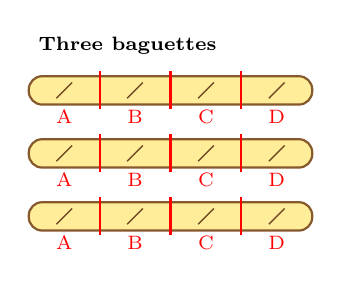
\begin{tikzpicture}[every node/.style={font=\scriptsize}]

% ---- Three baguettes, to share between teachers A, B, C and D ----
\node[dhead] at (0,0.75) {Three baguettes};
\foreach \y in {0,-0.8,-1.6} {\baguette{0}{\y}}
% --- Q8 answer: cut each baguette into quarters, one quarter each ---
\foreach \y in {0,-0.8,-1.6} {
  \bagcuts{\y}
  \baglabels{\y}{A}{B}{C}{D}
}

\end{tikzpicture}

\begin{pattern}{Pattern for Q4}
  $5-2$      & $3$\\
  $5-1$      & \ablank{$4$}\\
  $5-0$      & \ablank{$5$}\\
  $5-(-1)$   & \ablank{$6$}\\
  $5-(-2)$   & \ablank{$7$}
\end{pattern}

\column{0.64\textwidth}
\vspace{-1.5em}
\footnotesize
\begin{enumerate}\tightlist
{\setlength{\columnsep}{14pt}%
\begin{multicols}{3}
  \item $-4+9$ \ashow{$=5$}
  \columnbreak
  \item $-4-9$ \ashow{$=-13$}
  \columnbreak
  \item $6.05-2.8$ \ashow{$=3.25$}
\end{multicols}}
  \item Complete the pattern on the left. What is subtracting $-1$ the same as?
        \ashow{Adding $1$}
\begin{multicols}{2}
  \item $6+(-4)$ \ashow{$=6-4=2$}
  \columnbreak
  \item $-3-(-8)$ \ashow{$=-3+8=5$}
\end{multicols}
  \item It is \dC{5} at the foot of a mountain and \dC{-12} at the top. How much colder
        is the top? Write this as a subtraction.
        \ashow{$5-(-12)=17$ degrees}
  \item Three baguettes are shared equally between teachers A, B, C and D. Show on
        the diagram how to cut them. What fraction of a baguette does each teacher get?
        \ashow{Three quarters of a baguette}
\begin{multicols}{2}
  \item Write $3\div4$ as a fraction.
        \ashow{$\dfrac34$}
  \columnbreak
  \item Write $3\div4$ as a decimal.
        \ashow{$0.75$}
\end{multicols}
  \item (Challenge) Seven baguettes are shared equally between three teachers. Write
        each share as a division, a fraction and a recurring decimal.
        \ashow{$7\div3=\dfrac73=2.\dot{3}$}
\end{enumerate}
\end{columns}
\end{frame}

\begin{frame}[t]{Worked Solution: Retrieve and Connect 3, Question 1}
\hypertarget{work-st3}{}
\textbf{Question:} $-4+9$ \\
\awork{Solution: $-4+9 = 5$. \\
Start at $-4$ and move $9$ right.}
\end{frame}

\begin{frame}[t]{Worked Solution: Retrieve and Connect 3, Question 2}
\textbf{Question:} $-4-9$ \\
\awork{Solution: $-4-9 = -13$. \\
Start at $-4$ and move $9$ left.}
\end{frame}

\begin{frame}[t]{Worked Solution: Retrieve and Connect 3, Question 3}
\textbf{Question:} $6.05-2.8$ \\
\awork{Solution: Write $2.8$ as $2.80$. \\
$6.05 - 2.80 = 3.25$.}
\end{frame}

\begin{frame}[t]{Worked Solution: Retrieve and Connect 3, Question 4}
\textbf{Question:} Complete the pattern: $5-2=3$, $5-1=4$, $5-0=5$, $5-(-1)=\Box$, $5-(-2)=\Box$. What is subtracting $-1$ the same as? \\
\awork{Solution: The pattern increases by $1$ each time. \\
$5-(-1)=6$, $5-(-2)=7$. \\
Subtracting $-1$ is the same as adding $1$.}
\end{frame}

\begin{frame}[t]{Worked Solution: Retrieve and Connect 3, Question 5}
\textbf{Question:} $6+(-4)$ \\
\awork{Solution: $6+(-4) = 6-4 = 2$. \\
Adding a negative is the same as subtracting.}
\end{frame}

\begin{frame}[t]{Worked Solution: Retrieve and Connect 3, Question 6}
\textbf{Question:} $-3-(-8)$ \\
\awork{Solution: $-3-(-8) = -3+8 = 5$. \\
Subtracting a negative is the same as adding.}
\end{frame}

\begin{frame}[t]{Worked Solution: Retrieve and Connect 3, Question 7}
\textbf{Question:} It is $5^\circ$C at the foot of a mountain and $-12^\circ$C at the top. How much colder is the top? Write this as a subtraction. \\
\awork{Solution: Difference $= 5 - (-12) = 5 + 12 = 17$. \\
The top is $17$ degrees colder.}
\end{frame}

\begin{frame}[t]{Worked Solution: Retrieve and Connect 3, Question 8}
\textbf{Question:} Three baguettes are shared equally between teachers A, B, C and D. Show on the diagram how to cut them. What fraction of a baguette does each teacher get? \\
\awork{Solution: Cut each baguette into $4$ equal quarters. Each teacher gets $3$ quarters, which is $\frac{3}{4}$ of a baguette.}
\end{frame}

\begin{frame}[t]{Worked Solution: Retrieve and Connect 3, Question 9}
\textbf{Question:} Write $3\div4$ as a fraction. \\
\awork{Solution: $3\div4 = \frac{3}{4}$.}
\end{frame}

\begin{frame}[t]{Worked Solution: Retrieve and Connect 3, Question 10}
\textbf{Question:} Write $3\div4$ as a decimal. \\
\awork{Solution: $3\div4 = 0.75$.}
\end{frame}

\begin{frame}[t]{Worked Solution: Retrieve and Connect 3, Question 11}
\textbf{Question:} (Challenge) Seven baguettes are shared equally between three teachers. Write each share as a division, a fraction and a recurring decimal. \\
\awork{Solution: $7 \div 3 = \frac{7}{3} = 2.333\ldots = 2.\dot{3}$. \\
Each teacher gets $2.\dot{3}$ baguettes.}
\end{frame}

%------------------------------------------------------------------
% STARTER 4: Multiplying and dividing negative numbers
%------------------------------------------------------------------
\begin{frame}[t]{Retrieve and Connect: Multiplying \& Dividing Negatives}
\hypertarget{q-st4}{}
\begin{columns}[T,onlytextwidth]

\column{0.36\textwidth}
\vspace{-0.4em}
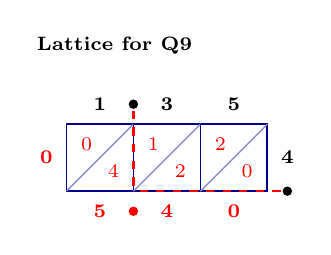
\begin{tikzpicture}[every node/.style={font=\scriptsize}]

% ---- Lattice for 1.35 x 4. The decimal point of 1.35 is marked on the top
% edge, and the decimal point of 4, which comes after the 4, at the bottom of
% the right-hand edge. ----
\node[dhead] at (0,1.0) {Lattice for Q9};
\begin{scope}[x=0.85cm, y=0.85cm, xshift=0.5cm]
\lgrid{3}{1}
\ltop{1}{1}\ltop{2}{3}\ltop{3}{5}
\lside{3}{1}{4}
\lpoint{1}{0.3}
\lpoint{3.3}{-1}
% --- Q9 answer ---
\lcell{1}{1}{0}{4}\lcell{2}{1}{1}{2}\lcell{3}{1}{2}{0}
\lleft{1}{0}
\lbot{1}{1}{5}\lbot{1}{2}{4}\lbot{1}{3}{0}
% the two decimal points meet on the bottom edge, so the point in the answer
% goes between the 5 and the 4
\draw[ans, dashed] (1,0.2) -- (1,-1);
\draw[ans, dashed] (3.2,-1) -- (1,-1);
\lpoint[ans]{1}{-1.3}
\end{scope}

\end{tikzpicture}

\orrule
\begin{scaling}
  $1.35\times100=135$\\
  $135\times4=\ablank{540}$\\
  We multiplied by $100$, so\\
  $1.35\times4=\ablank{5.40}$
\end{scaling}

\begin{pattern}{Pattern for Q4}
  $(-3)\times2$      & $-6$\\
  $(-3)\times1$      & $-3$\\
  $(-3)\times0$      & \ablank{$0$}\\
  $(-3)\times(-1)$   & \ablank{$3$}\\
  $(-3)\times(-2)$   & \ablank{$6$}
\end{pattern}

\column{0.64\textwidth}
\vspace{-1.5em}
\footnotesize
\begin{enumerate}\tightlist
\begin{multicols}{2}
  \item $-7+3$ \ashow{$=-4$}
  \columnbreak
  \item $4-(-6)$ \ashow{$=10$}
\end{multicols}
  \item Use bus stop division to work out $5\div6$.
        \ashow{$0.8\dot{3}$}
  \item Complete the pattern on the left. Is a negative number multiplied by a
        negative number positive or negative?
        \ashow{Positive}
\begin{multicols}{2}
  \item $5\times(-4)$ \ashow{$=-20$}
  \columnbreak
  \item $(-6)\times(-3)$ \ashow{$=18$}
\end{multicols}
\begin{multicols}{2}
  \item $-20\div5$ \ashow{$=-4$}
  \columnbreak
  \item $-18\div(-2)$ \ashow{$=9$}
\end{multicols}
  \item Find the cost of $4$ baguettes at £$1.35$ each. Use one of the two methods on
        the left.
        \ashow{£$5.40$}
  \item The staff room fund has £$5.00$, and pays for the four baguettes. What is its
        balance now?
        \ashow{$5.00-5.40=-0.40$, so $-$£$0.40$}
  \item $-4.8\div0.6=\dfrac{-4.8}{0.6}=\dfrac{-4.8\times10}{0.6\times10}
        =\dfrac{\ablank{-48}}{\ablank{6}}=\ablank{-8}$
  \item[] \vspace{3pt}(Challenge)
\begin{multicols}{2}
  \item $(-0.3)\times(-0.4)$ \ashow{$=0.12$}
  \columnbreak
  \item $-1.2\div(-0.04)$ \ashow{$=\dfrac{-120}{-4}=30$}
\end{multicols}
\end{enumerate}
\end{columns}
\end{frame}

\begin{frame}[t]{Worked Solution: Retrieve and Connect 4, Question 1}
\hypertarget{work-st4}{}
\textbf{Question:} $-7+3$ \\
\awork{Solution: $-7+3 = -4$. \\
Start at $-7$ and move $3$ right.}
\end{frame}

\begin{frame}[t]{Worked Solution: Retrieve and Connect 4, Question 2}
\textbf{Question:} $4-(-6)$ \\
\awork{Solution: $4-(-6) = 4+6 = 10$. \\
Subtracting a negative is the same as adding.}
\end{frame}

\begin{frame}[t]{Worked Solution: Retrieve and Connect 4, Question 3}
\textbf{Question:} Use bus stop division to work out $5\div6$. \\
\awork{Solution: $5 \div 6 = 0.8333\ldots$ \\
The remainder repeats, so $5\div6 = 0.8\dot{3}$.}
\end{frame}

\begin{frame}[t]{Worked Solution: Retrieve and Connect 4, Question 4}
\textbf{Question:} Complete the pattern: $(-3)\times2=-6$, $(-3)\times1=-3$, $(-3)\times0=\Box$, $(-3)\times(-1)=\Box$, $(-3)\times(-2)=\Box$. Is a negative number multiplied by a negative number positive or negative? \\
\awork{Solution: The pattern increases by $3$ each time. \\
$(-3)\times0=0$, $(-3)\times(-1)=3$, $(-3)\times(-2)=6$. \\
A negative times a negative is positive.}
\end{frame}

\begin{frame}[t]{Worked Solution: Retrieve and Connect 4, Question 5}
\textbf{Question:} $5\times(-4)$ \\
\awork{Solution: $5\times(-4) = -20$. \\
Positive times negative gives a negative.}
\end{frame}

\begin{frame}[t]{Worked Solution: Retrieve and Connect 4, Question 6}
\textbf{Question:} $(-6)\times(-3)$ \\
\awork{Solution: $(-6)\times(-3) = 18$. \\
Negative times negative gives a positive.}
\end{frame}

\begin{frame}[t]{Worked Solution: Retrieve and Connect 4, Question 7}
\textbf{Question:} $-20\div5$ \\
\awork{Solution: $-20\div5 = -4$. \\
Negative divided by positive gives a negative.}
\end{frame}

\begin{frame}[t]{Worked Solution: Retrieve and Connect 4, Question 8}
\textbf{Question:} $-18\div(-2)$ \\
\awork{Solution: $-18\div(-2) = 9$. \\
Negative divided by negative gives a positive.}
\end{frame}

\begin{frame}[t]{Worked Solution: Retrieve and Connect 4, Question 9}
\textbf{Question:} Find the cost of $4$ baguettes at £$1.35$ each. Use one of the two methods on the left. \\
\awork{Solution: Scaling method: $1.35\times100=135$, $135\times4=540$, so $1.35\times4=5.40$. \\
Cost is £$5.40$.}
\end{frame}

\begin{frame}[t]{Worked Solution: Retrieve and Connect 4, Question 10}
\textbf{Question:} The staff room fund has £$5.00$, and pays for the four baguettes. What is its balance now? \\
\awork{Solution: $5.00 - 5.40 = -0.40$. \\
The balance is $-$£$0.40$.}
\end{frame}

\begin{frame}[t]{Worked Solution: Retrieve and Connect 4, Question 11}
\textbf{Question:} $-4.8\div0.6=\dfrac{-4.8}{0.6}=\dfrac{-4.8\times10}{0.6\times10}=\dfrac{\Box}{\Box}=\Box$ \\
\awork{Solution: Multiply numerator and denominator by $10$: \\
$\dfrac{-4.8\times10}{0.6\times10} = \dfrac{-48}{6} = -8$.}
\end{frame}

\begin{frame}[t]{Worked Solution: Retrieve and Connect 4, Question 12}
\textbf{Question:} (Challenge) $(-0.3)\times(-0.4)$ \\
\awork{Solution: $(-0.3)\times(-0.4) = 0.12$. \\
Negative times negative is positive.}
\end{frame}

\begin{frame}[t]{Worked Solution: Retrieve and Connect 4, Question 13}
\textbf{Question:} (Challenge) $-1.2\div(-0.04)$ \\
\awork{Solution: $-1.2\div(-0.04) = \dfrac{-1.2}{-0.04} = \dfrac{-120}{-4} = 30$.}
\end{frame}

%------------------------------------------------------------------
% STARTER 5: Squares, cubes, square roots and cube roots
%------------------------------------------------------------------
\begin{frame}[t]{Retrieve and Connect: Squares, Cubes \& Roots}
\hypertarget{q-st5}{}
\begin{columns}[T,onlytextwidth]

\column{0.36\textwidth}
\vspace{-0.4em}
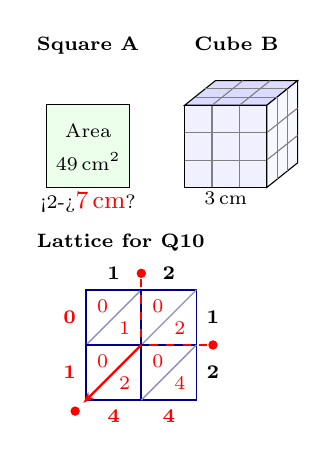
\begin{tikzpicture}[every node/.style={font=\scriptsize}]

% ---- Square A, with area 49 cm^2 ----
\node[dhead] at (0,0.75) {Square A};
\draw[fill=green!8] (0.25,-1.05) rectangle (1.3,0);
\node at (0.775,-0.33) {Area};
\node at (0.775,-0.72) {$49$\,cm$^2$};
% --- Q4 answer: the side length, where the question mark was ---
\node[below, inner sep=1.5pt] at (0.775,-1.05) {\ashowq{$7$\,cm}};

% ---- Cube B: 3 by 3 by 3 centimetre cubes, drawn in oblique projection ----
\begin{scope}[xshift=2.0cm, yshift=-1.05cm, scale=0.87]
\node[dhead] at (0,2.1) {Cube B};
% one centimetre along the front is 0.4, and one centimetre of depth is (0.15,0.12)
\draw[fill=blue!6]  (0,0) rectangle (1.2,1.2);
\draw[fill=blue!14] (0,1.2) -- (0.45,1.56) -- (1.65,1.56) -- (1.2,1.2) -- cycle;
\draw[fill=blue!3]  (1.2,0) -- (1.65,0.36) -- (1.65,1.56) -- (1.2,1.2) -- cycle;
\foreach \i in {1,2} {
  \draw[black!50] ({0.4*\i},0) -- ({0.4*\i},1.2);
  \draw[black!50] (0,{0.4*\i}) -- (1.2,{0.4*\i});
  \draw[black!50] ({0.4*\i},1.2) -- ({0.4*\i+0.45},1.56);
  \draw[black!50] ({0.15*\i},{1.2+0.12*\i}) -- ({1.2+0.15*\i},{1.2+0.12*\i});
  \draw[black!50] ({1.2+0.15*\i},{0.12*\i}) -- ({1.2+0.15*\i},{1.2+0.12*\i});
  \draw[black!50] (1.2,{0.4*\i}) -- (1.65,{0.4*\i+0.36});
}
\draw (0,0) rectangle (1.2,1.2);
\node[below, inner sep=1.5pt] at (0.6,0) {$3$\,cm};
\end{scope}

% ---- Lattice for 1.2 x 1.2. Pupils mark the decimal points themselves. ----
\node[dhead] at (0,-1.75) {Lattice for Q10};
\begin{scope}[x=0.7cm, y=0.7cm, xshift=0.75cm, yshift=-2.35cm]
\lgrid{2}{2}
\ltop{1}{1}\ltop{2}{2}
\lside{2}{1}{1}\lside{2}{2}{2}
% --- Q10 answer ---
\lcell{1}{1}{0}{1}\lcell{2}{1}{0}{2}
\lcell{1}{2}{0}{2}\lcell{2}{2}{0}{4}
\lleft{1}{0}\lleft{2}{1}
\lbot{2}{1}{4}\lbot{2}{2}{4}
% the decimal points meet in the middle; the diagonal leaves at the corner
\lpoint[ans]{1}{0.3}
\lpoint[ans]{2.3}{-1}
\draw[ans, dashed] (1,0.2) -- (1,-1);
\draw[ans, dashed] (2.2,-1) -- (1,-1);
\draw[ans, -{Stealth[length=4pt]}] (1,-1) -- (-0.05,-2.05);
\lpoint[ans]{-0.2}{-2.2}
\end{scope}

\end{tikzpicture}

\orrule
\begin{scaling}
  $1.2\times10=12$\\
  $12\times12=\ablank{144}$\\
  We multiplied by $10\times10$, so\\
  $1.2^2=\ablank{1.44}$
\end{scaling}

\column{0.64\textwidth}
\vspace{-1.5em}
\footnotesize
\begin{enumerate}\tightlist
{\setlength{\columnsep}{14pt}%
\begin{multicols}{3}
  \item $(-4)\times(-5)$ \ashow{$=20$}
  \columnbreak
  \item $-24\div6$ \ashow{$=-4$}
  \columnbreak
  \item Round $7.482$ to $1$ d.p.
        \ashow{$7.5$}
\end{multicols}}
  \item Square A has area $49$\,cm$^2$. Find its side length, using $\sqrt{\phantom{x}}$.
        \ashow{$\sqrt{49}=7$\,cm}
  \item Cube B is made of centimetre cubes. Find its volume, written as a power.
        \ashow{$3^3=27$\,cm$^3$}
\begin{multicols}{4}
  \item $6^2$ \ashow{$=36$}
  \columnbreak
  \item $4^3$ \ashow{$=64$}
  \columnbreak
  \item $\sqrt{81}$ \ashow{$=9$}
  \columnbreak
  \item $\sqrt[3]{1000}$ \ashow{$=10$}
\end{multicols}
  \item Work out $1.2^2=1.2\times1.2$ using one method on the left. On the lattice,
        mark the decimal points yourself.
        \ashow{$1.44$}
\begin{multicols}{2}
  \item $(-3)^2$ \ashow{$=9$}
  \columnbreak
  \item $(-2)^3$ \ashow{$=-8$}
\end{multicols}
\begin{multicols}{2}
  \item (Challenge) Find two numbers whose square is $64$.
        \ashow{$8$ and $-8$}
  \columnbreak
  \item (Challenge) Is there a number whose square is $-64$?
        \ashow{No: a square is never negative.}
\end{multicols}
\end{enumerate}
\end{columns}
\end{frame}

\begin{frame}[t]{Worked Solution: Retrieve and Connect 5, Question 1}
\hypertarget{work-st5}{}
\textbf{Question:} $(-4)\times(-5)$ \\
\awork{Solution: $(-4)\times(-5) = 20$. \\
Negative times negative is positive.}
\end{frame}

\begin{frame}[t]{Worked Solution: Retrieve and Connect 5, Question 2}
\textbf{Question:} $-24\div6$ \\
\awork{Solution: $-24\div6 = -4$. \\
Negative divided by positive is negative.}
\end{frame}

\begin{frame}[t]{Worked Solution: Retrieve and Connect 5, Question 3}
\textbf{Question:} Round $7.482$ to $1$ d.p. \\
\awork{Solution: The first decimal place is $4$. The next digit is $8$, so round up. \\
$7.482$ rounded to $1$ d.p. is $7.5$.}
\end{frame}

\begin{frame}[t]{Worked Solution: Retrieve and Connect 5, Question 4}
\textbf{Question:} Square A has area $49$\,cm$^2$. Find its side length, using $\sqrt{\phantom{x}}$. \\
\awork{Solution: The side length is $\sqrt{49} = 7$\,cm.}
\end{frame}

\begin{frame}[t]{Worked Solution: Retrieve and Connect 5, Question 5}
\textbf{Question:} Cube B is made of centimetre cubes. Find its volume, written as a power. \\
\awork{Solution: The cube is $3$ by $3$ by $3$, so volume $= 3^3 = 27$\,cm$^3$.}
\end{frame}

\begin{frame}[t]{Worked Solution: Retrieve and Connect 5, Question 6}
\textbf{Question:} $6^2$ \\
\awork{Solution: $6^2 = 36$.}
\end{frame}

\begin{frame}[t]{Worked Solution: Retrieve and Connect 5, Question 7}
\textbf{Question:} $4^3$ \\
\awork{Solution: $4^3 = 4\times4\times4 = 64$.}
\end{frame}

\begin{frame}[t]{Worked Solution: Retrieve and Connect 5, Question 8}
\textbf{Question:} $\sqrt{81}$ \\
\awork{Solution: $\sqrt{81} = 9$, because $9\times9=81$.}
\end{frame}

\begin{frame}[t]{Worked Solution: Retrieve and Connect 5, Question 9}
\textbf{Question:} $\sqrt[3]{1000}$ \\
\awork{Solution: $\sqrt[3]{1000} = 10$, because $10^3=1000$.}
\end{frame}

\begin{frame}[t]{Worked Solution: Retrieve and Connect 5, Question 10}
\textbf{Question:} Work out $1.2^2=1.2\times1.2$ using one method on the left. On the lattice, mark the decimal points yourself. \\
\awork{Solution: Using scaling: $1.2\times10=12$, $12\times12=144$. \\
We multiplied by $10\times10=100$, so $1.2^2 = 1.44$.}
\end{frame}

\begin{frame}[t]{Worked Solution: Retrieve and Connect 5, Question 11}
\textbf{Question:} $(-3)^2$ \\
\awork{Solution: $(-3)^2 = (-3)\times(-3) = 9$.}
\end{frame}

\begin{frame}[t]{Worked Solution: Retrieve and Connect 5, Question 12}
\textbf{Question:} $(-2)^3$ \\
\awork{Solution: $(-2)^3 = (-2)\times(-2)\times(-2) = 4\times(-2) = -8$.}
\end{frame}

\begin{frame}[t]{Worked Solution: Retrieve and Connect 5, Question 13}
\textbf{Question:} (Challenge) Find two numbers whose square is $64$. \\
\awork{Solution: The numbers are $8$ and $-8$, because $8^2=64$ and $(-8)^2=64$.}
\end{frame}

\begin{frame}[t]{Worked Solution: Retrieve and Connect 5, Question 14}
\textbf{Question:} (Challenge) Is there a number whose square is $-64$? \\
\awork{Solution: No. The square of any real number is never negative.}
\end{frame}

%------------------------------------------------------------------
% STARTER 6: Index notation, powers of 10, and estimating square roots
%------------------------------------------------------------------
\begin{frame}[t]{Retrieve and Connect: Powers \& Estimating Roots}
\hypertarget{q-st6}{}
\begin{columns}[T,onlytextwidth]

\column{0.36\textwidth}
\vspace{-0.4em}
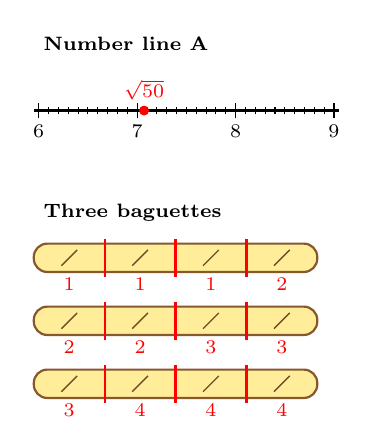
\begin{tikzpicture}[every node/.style={font=\scriptsize}]

% ---- Number line A: 6 to 9 in tenths ----
\begin{scope}[x=1.25cm, shift={(-5.95,0)}]
\node[dhead] at (5.95,0.85) {Number line A};
\draw[thick] (5.95,0) -- (9.05,0);
\foreach \v in {6,6.1,...,9.01} \draw (\v,-0.05) -- (\v,0.05);
\foreach \v in {6,...,9} {
  \draw (\v,-0.1) -- (\v,0.1);
  \node[nlab] at (\v,-0.1) {$\v$};
}
% --- Q8 answer: sqrt 50 is just above 7, because 50 is just above 49 ---
\fill[ans] (7.07,0) circle (1.8pt);
\node[vans, above, inner sep=1.5pt] at (7.07,0.07) {$\sqrt{50}$};
\end{scope}

% ---- Three baguettes, to share out 0.75 of a baguette at a time ----
\begin{scope}[yshift=-2.05cm]
\node[dhead] at (0,0.75) {Three baguettes};
\foreach \y in {0,-0.8,-1.6} {\baguette{0}{\y}}
% --- Q11 answer: quarters, handed out three at a time to teachers 1 to 4 ---
\foreach \y in {0,-0.8,-1.6} {\bagcuts{\y}}
\baglabels{0}{1}{1}{1}{2}
\baglabels{-0.8}{2}{2}{3}{3}
\baglabels{-1.6}{3}{4}{4}{4}
\end{scope}

\end{tikzpicture}

\column{0.64\textwidth}
\vspace{-1.5em}
\footnotesize
\begin{enumerate}\tightlist
\begin{multicols}{2}
  \item $7^2$ \ashow{$=49$}
  \columnbreak
  \item $\sqrt{144}$ \ashow{$=12$}
\end{multicols}
\begin{multicols}{2}
  \item $-2.4+5$ \ashow{$=2.6$}
  \columnbreak
  \item $-3\times(-1.5)$ \ashow{$=4.5$}
\end{multicols}
  \item Write $2\times2\times2\times2\times2$ as a power, and work it out. Write $<$ or
        $>$ between $2^5$ and $5^2$.
        \ashow{$2^5=32>25$}
\begin{multicols}{2}
  \item $10^4$ \ashow{$=10\,000$}
  \columnbreak
  \item $3.7\times10^3$ \ashow{$=3700$}
\end{multicols}
  \item Complete \; $\ablank{7}<\sqrt{50}<\ablank{8}$, \; and mark $\sqrt{50}$ on
        number line A.
        \ashow{Just above $7$, as $50$ is near $49$}
\begin{multicols}{2}
  \item $0.7^2$ \ashow{$=0.49$}
  \columnbreak
  \item $\sqrt{0.49}$ \ashow{$=0.7$}
\end{multicols}
  \item Each teacher eats $0.75$ of a baguette. Show on the diagram how many teachers
        $3$ baguettes can feed. \;
        $3\div0.75=\dfrac{3}{0.75}=\dfrac{\ablank{300}}{\ablank{75}}=\ablank{4}$
  \vspace{3pt}\item (Challenge) A baguette is $0.6$\,m long. Each teacher's portion is $0.15$\,m
        long. How many portions can be cut from $3$ baguettes?
        \ashow{$0.6\div0.15=\dfrac{60}{15}=4$; \; $3\times4=12$ portions}
\end{enumerate}
\end{columns}
\end{frame}

\begin{frame}[t]{Worked Solution: Retrieve and Connect 6, Question 1}
\hypertarget{work-st6}{}
\textbf{Question:} $7^2$ \\
\awork{Solution: $7^2 = 7\times7 = 49$.}
\end{frame}

\begin{frame}[t]{Worked Solution: Retrieve and Connect 6, Question 2}
\textbf{Question:} $\sqrt{144}$ \\
\awork{Solution: $\sqrt{144} = 12$, because $12\times12=144$.}
\end{frame}

\begin{frame}[t]{Worked Solution: Retrieve and Connect 6, Question 3}
\textbf{Question:} $-2.4+5$ \\
\awork{Solution: $-2.4+5 = 2.6$. \\
Start at $-2.4$ and move $5$ right.}
\end{frame}

\begin{frame}[t]{Worked Solution: Retrieve and Connect 6, Question 4}
\textbf{Question:} $-3\times(-1.5)$ \\
\awork{Solution: $-3\times(-1.5) = 4.5$. \\
Negative times negative is positive.}
\end{frame}

\begin{frame}[t]{Worked Solution: Retrieve and Connect 6, Question 5}
\textbf{Question:} Write $2\times2\times2\times2\times2$ as a power, and work it out. Write $<$ or $>$ between $2^5$ and $5^2$. \\
\awork{Solution: $2\times2\times2\times2\times2 = 2^5 = 32$. \\
$5^2 = 25$. \\
$32 > 25$, so $2^5 > 5^2$.}
\end{frame}

\begin{frame}[t]{Worked Solution: Retrieve and Connect 6, Question 6}
\textbf{Question:} $10^4$ \\
\awork{Solution: $10^4 = 10\times10\times10\times10 = 10\,000$.}
\end{frame}

\begin{frame}[t]{Worked Solution: Retrieve and Connect 6, Question 7}
\textbf{Question:} $3.7\times10^3$ \\
\awork{Solution: $3.7\times10^3 = 3.7\times1000 = 3700$.}
\end{frame}

\begin{frame}[t]{Worked Solution: Retrieve and Connect 6, Question 8}
\textbf{Question:} Complete $7<\sqrt{50}<8$, and mark $\sqrt{50}$ on number line A. \\
\awork{Solution: $7^2=49$ and $8^2=64$, and $50$ is between $49$ and $64$. \\
So $\sqrt{50}$ is between $7$ and $8$, just above $7$.}
\end{frame}

\begin{frame}[t]{Worked Solution: Retrieve and Connect 6, Question 9}
\textbf{Question:} $0.7^2$ \\
\awork{Solution: $0.7^2 = 0.7\times0.7 = 0.49$.}
\end{frame}

\begin{frame}[t]{Worked Solution: Retrieve and Connect 6, Question 10}
\textbf{Question:} $\sqrt{0.49}$ \\
\awork{Solution: $\sqrt{0.49} = 0.7$, because $0.7^2=0.49$.}
\end{frame}

\begin{frame}[t]{Worked Solution: Retrieve and Connect 6, Question 11}
\textbf{Question:} Each teacher eats $0.75$ of a baguette. Show on the diagram how many teachers $3$ baguettes can feed. \\
\awork{Solution: $3 \div 0.75 = \dfrac{3}{0.75} = \dfrac{300}{75} = 4$. \\
So $3$ baguettes can feed $4$ teachers.}
\end{frame}

\begin{frame}[t]{Worked Solution: Retrieve and Connect 6, Question 12}
\textbf{Question:} (Challenge) A baguette is $0.6$\,m long. Each teacher's portion is $0.15$\,m long. How many portions can be cut from $3$ baguettes? \\
\awork{Solution: One baguette gives $0.6 \div 0.15 = \dfrac{60}{15} = 4$ portions. \\
Three baguettes give $3\times4 = 12$ portions.}
\end{frame}

%------------------------------------------------------------------
% STARTER 7: BIDMAS
%------------------------------------------------------------------
\begin{frame}[t]{Retrieve and Connect: BIDMAS}
\hypertarget{q-st7}{}
\begin{columns}[T,onlytextwidth]

\column{0.36\textwidth}
\vspace{-0.4em}
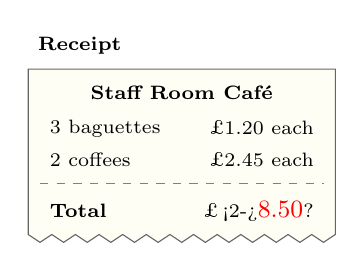
\begin{tikzpicture}[every node/.style={font=\scriptsize}]

% ---- A receipt from the staff room café, with a torn bottom edge ----
\node[dhead] at (0,0.3) {Receipt};
\draw[fill=yellow!4, draw=black!60]
  (0,0) -- (3.9,0) -- (3.9,-2.1)
  \foreach \i in {1,...,13} { -- ({3.9-0.3*\i+0.15},-2.2) -- ({3.9-0.3*\i},-2.1) }
  -- cycle;
\node[font=\scriptsize\bfseries] at (1.95,-0.3) {Staff Room Café};
\node[anchor=west] at (0.15,-0.75) {$3$ baguettes};
\node[anchor=east] at (3.75,-0.75) {£$1.20$ each};
\node[anchor=west] at (0.15,-1.15) {$2$ coffees};
\node[anchor=east] at (3.75,-1.15) {£$2.45$ each};
\draw[black!50, dashed] (0.15,-1.45) -- (3.75,-1.45);
\node[anchor=west, font=\scriptsize\bfseries] at (0.15,-1.8) {Total};
% --- Q9 answer: the total ---
\node[anchor=east] at (3.75,-1.8)
  {£\,\ashowq{$8.50$}};

\end{tikzpicture}

\column{0.64\textwidth}
\vspace{-1.5em}
\footnotesize
\begin{enumerate}\tightlist
\begin{multicols}{2}
  \item $4^2-\sqrt9$ \ashow{$=16-3=13$}
  \columnbreak
  \item $(-12)\div2\times3$ \ashow{$=-6\times3=-18$}
\end{multicols}
\begin{multicols}{2}
  \item $3+4\times5$ \ashow{$=3+20=23$}
  \columnbreak
  \item $(3+4)\times5$ \ashow{$=7\times5=35$}
\end{multicols}
\begin{multicols}{2}
  \item $20-12\div3$ \ashow{$=20-4=16$}
  \columnbreak
  \item $(20-12)\div3$, as a recurring decimal
        \ashow{$=8\div3=2.\dot{6}$}
\end{multicols}
\begin{multicols}{2}
  \item $\dfrac{18+6}{4}$ \ashow{$=\dfrac{24}{4}=6$}
  \columnbreak
  \item $18+6\div4$ \ashow{$=18+1.5=19.5$}
\end{multicols}
  \item Three teachers buy the items on the receipt. Write one calculation for the total
        cost, and work it out.
        \ashow{$3\times1.20+2\times2.45=3.60+4.90=$ £$8.50$}
  \item They share the cost equally. Write one calculation, with brackets, for each
        share, to the nearest penny.
        \ashow{$(3\times1.20+2\times2.45)\div3=2.833\ldots\approx$ £$2.83$}
  \item[] (Challenge) Put brackets into $2+6\times5-3$ to make each number.
\begin{multicols}{2}
  \item $16$ \ashow{\; $(2+6)\times(5-3)$}
  \columnbreak
  \item $37$ \ashow{\; $(2+6)\times5-3$}
\end{multicols}
\end{enumerate}
\end{columns}
\end{frame}

\begin{frame}[t]{Worked Solution: Retrieve and Connect 7, Question 1}
\hypertarget{work-st7}{}
\textbf{Question:} $4^2-\sqrt9$ \\
\awork{Solution: $4^2=16$ and $\sqrt9=3$. \\
$16 - 3 = 13$.}
\end{frame}

\begin{frame}[t]{Worked Solution: Retrieve and Connect 7, Question 2}
\textbf{Question:} $(-12)\div2\times3$ \\
\awork{Solution: Work left to right: $(-12)\div2 = -6$. \\
$-6\times3 = -18$.}
\end{frame}

\begin{frame}[t]{Worked Solution: Retrieve and Connect 7, Question 3}
\textbf{Question:} $3+4\times5$ \\
\awork{Solution: Multiplication before addition. \\
$4\times5=20$, then $3+20=23$.}
\end{frame}

\begin{frame}[t]{Worked Solution: Retrieve and Connect 7, Question 4}
\textbf{Question:} $(3+4)\times5$ \\
\awork{Solution: Brackets first: $3+4=7$. \\
$7\times5=35$.}
\end{frame}

\begin{frame}[t]{Worked Solution: Retrieve and Connect 7, Question 5}
\textbf{Question:} $20-12\div3$ \\
\awork{Solution: Division before subtraction. \\
$12\div3=4$, then $20-4=16$.}
\end{frame}

\begin{frame}[t]{Worked Solution: Retrieve and Connect 7, Question 6}
\textbf{Question:} $(20-12)\div3$, as a recurring decimal \\
\awork{Solution: Brackets first: $20-12=8$. \\
$8\div3 = 2.666\ldots = 2.\dot{6}$.}
\end{frame}

\begin{frame}[t]{Worked Solution: Retrieve and Connect 7, Question 7}
\textbf{Question:} $\dfrac{18+6}{4}$ \\
\awork{Solution: The fraction bar means division, so first $18+6=24$. \\
$24\div4=6$.}
\end{frame}

\begin{frame}[t]{Worked Solution: Retrieve and Connect 7, Question 8}
\textbf{Question:} $18+6\div4$ \\
\awork{Solution: Division before addition. \\
$6\div4=1.5$, then $18+1.5=19.5$.}
\end{frame}

\begin{frame}[t]{Worked Solution: Retrieve and Connect 7, Question 9}
\textbf{Question:} Three teachers buy $3$ baguettes at £$1.20$ each and $2$ coffees at £$2.45$ each. Write one calculation for the total cost, and work it out. \\
\awork{Solution: Total $= 3\times1.20 + 2\times2.45$. \\
$= 3.60 + 4.90 = 8.50$. \\
Total cost is £$8.50$.}
\end{frame}

\begin{frame}[t]{Worked Solution: Retrieve and Connect 7, Question 10}
\textbf{Question:} They share the cost equally. Write one calculation, with brackets, for each share, to the nearest penny. \\
\awork{Solution: Each share $= (3\times1.20 + 2\times2.45)\div3$. \\
$= 8.50 \div 3 = 2.8333\ldots \approx £2.83$.}
\end{frame}

\begin{frame}[t]{Worked Solution: Retrieve and Connect 7, Question 11}
\textbf{Question:} (Challenge) Put brackets into $2+6\times5-3$ to make $16$. \\
\awork{Solution: $(2+6)\times(5-3) = 8\times2 = 16$.}
\end{frame}

\begin{frame}[t]{Worked Solution: Retrieve and Connect 7, Question 12}
\textbf{Question:} (Challenge) Put brackets into $2+6\times5-3$ to make $37$. \\
\awork{Solution: $(2+6)\times5 - 3 = 8\times5 - 3 = 40 - 3 = 37$.}
\end{frame}

%------------------------------------------------------------------
% STARTER 8: BIDMAS with powers, roots and negative numbers
%------------------------------------------------------------------
\begin{frame}[t]{Retrieve and Connect: BIDMAS with Powers \& Negatives}
\hypertarget{q-st8}{}
\begin{columns}[T,onlytextwidth]

\column{0.36\textwidth}
\vspace{-0.4em}
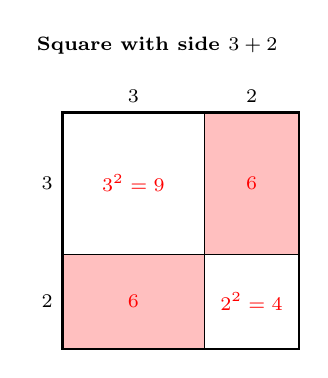
\begin{tikzpicture}[every node/.style={font=\scriptsize}]

% ---- A square with side 3 + 2, split into 3 by 3, 2 by 2 and two 3 by 2 parts.
% One unit is 0.6 cm. ----
\node[dhead] at (0,0.75) {Square with side $3+2$};
\begin{scope}[x=0.6cm, y=0.6cm, xshift=0.45cm, yshift=-3.1cm]
% --- Q10 answer: the two 3 by 2 rectangles that 3^2 + 2^2 leaves out ---
\fill[ansfill, red!25] (3,2) rectangle (5,5);
\fill[ansfill, red!25] (0,0) rectangle (3,2);
\draw[thick] (0,0) rectangle (5,5);
\draw (3,0) -- (3,5);
\draw (0,2) -- (5,2);
\node[above] at (1.5,5) {$3$};
\node[above] at (4,5)   {$2$};
\node[left]  at (0,3.5) {$3$};
\node[left]  at (0,1)   {$2$};
\node[vans] at (1.5,3.5) {$3^2=9$};
\node[vans] at (4,3.5)   {$6$};
\node[vans] at (1.5,1)   {$6$};
\node[vans] at (4,1)     {$2^2=4$};
\end{scope}

\end{tikzpicture}

\column{0.64\textwidth}
\vspace{-1.5em}
\footnotesize
\begin{enumerate}\tightlist
\begin{multicols}{2}
  \item $5+3\times2.5$ \ashow{$=5+7.5=12.5$}
  \columnbreak
  \item $\sqrt{64}-2^3$ \ashow{$=8-8=0$}
\end{multicols}
\begin{multicols}{2}
  \item $-3^2$ \ashow{$=-9$}
  \columnbreak
  \item $(-3)^2$ \ashow{$=9$}
\end{multicols}
  \item Explain why your answers to Q3 and Q4 are different.
        \ashow{In $-3^2$ only the $3$ is squared.}
\begin{multicols}{2}
  \item $2\times5^2$ \ashow{$=2\times25=50$}
  \columnbreak
  \item $(2\times5)^2$ \ashow{$=10^2=100$}
\end{multicols}
\begin{multicols}{2}
  \item $(3+2)^2$ \ashow{$=25$}
  \columnbreak
  \item $3^2+2^2$ \ashow{$=13$}
\end{multicols}
  \item Use the diagram to explain why your answers to Q8 and Q9 are different.
        \ashow{$3^2+2^2$ leaves out the two $3\times2$ rectangles.}
  \vspace{3pt}\item $\dfrac{4^2+2^3}{-9}$, as a recurring decimal
        \ashow{$=\dfrac{24}{-9}=-2.\dot{6}$}
\vspace{3pt}
\begin{multicols}{2}
  \item $\sqrt{36+64}$ \ashow{$=\sqrt{100}=10$}
  \columnbreak
  \item $\sqrt{36}+\sqrt{64}$ \ashow{$=6+8=14$}
\end{multicols}
  \item[] (Challenge) Use $2$, $3$ and $4$ once each, with any operations, powers or
        brackets, to make each number.
\begin{multicols}{2}
  \item $-10$ \ashow{\; for example $2-3\times4$}
  \columnbreak
  \item $36$ \ashow{\; for example $3^2\times4$}
\end{multicols}
\end{enumerate}
\end{columns}
\end{frame}

\begin{frame}[t]{Worked Solution: Retrieve and Connect 8, Question 1}
\hypertarget{work-st8}{}
\textbf{Question:} $5+3\times2.5$ \\
\awork{Solution: Multiplication before addition. \\
$3\times2.5 = 7.5$, then $5+7.5 = 12.5$.}
\end{frame}

\begin{frame}[t]{Worked Solution: Retrieve and Connect 8, Question 2}
\textbf{Question:} $\sqrt{64}-2^3$ \\
\awork{Solution: $\sqrt{64}=8$ and $2^3=8$. \\
$8-8=0$.}
\end{frame}

\begin{frame}[t]{Worked Solution: Retrieve and Connect 8, Question 3}
\textbf{Question:} $-3^2$ \\
\awork{Solution: The exponent applies only to $3$. \\
$-3^2 = -(3^2) = -9$.}
\end{frame}

\begin{frame}[t]{Worked Solution: Retrieve and Connect 8, Question 4}
\textbf{Question:} $(-3)^2$ \\
\awork{Solution: The exponent applies to $-3$. \\
$(-3)^2 = (-3)\times(-3) = 9$.}
\end{frame}

\begin{frame}[t]{Worked Solution: Retrieve and Connect 8, Question 5}
\textbf{Question:} Explain why your answers to Q3 and Q4 are different. \\
\awork{Solution: In $-3^2$, only the $3$ is squared, so it is $-(3\times3)=-9$. \\
In $(-3)^2$, the whole of $-3$ is squared, so it is $(-3)\times(-3)=9$.}
\end{frame}

\begin{frame}[t]{Worked Solution: Retrieve and Connect 8, Question 6}
\textbf{Question:} $2\times5^2$ \\
\awork{Solution: $5^2 = 25$. \\
$2\times25 = 50$.}
\end{frame}

\begin{frame}[t]{Worked Solution: Retrieve and Connect 8, Question 7}
\textbf{Question:} $(2\times5)^2$ \\
\awork{Solution: Brackets first: $2\times5=10$. \\
$10^2 = 100$.}
\end{frame}

\begin{frame}[t]{Worked Solution: Retrieve and Connect 8, Question 8}
\textbf{Question:} $(3+2)^2$ \\
\awork{Solution: Brackets first: $3+2=5$. \\
$5^2 = 25$.}
\end{frame}

\begin{frame}[t]{Worked Solution: Retrieve and Connect 8, Question 9}
\textbf{Question:} $3^2+2^2$ \\
\awork{Solution: $3^2=9$ and $2^2=4$. \\
$9+4=13$.}
\end{frame}

\begin{frame}[t]{Worked Solution: Retrieve and Connect 8, Question 10}
\textbf{Question:} Use the diagram to explain why your answers to Q8 and Q9 are different. \\
\awork{Solution: $(3+2)^2$ is the area of the whole square of side $5$, which is $25$. \\
$3^2+2^2$ adds only the two small squares ($9$ and $4$), but leaves out the two $3\times2$ rectangles (each $6$). So $3^2+2^2=13 \neq 25$.}
\end{frame}

\begin{frame}[t]{Worked Solution: Retrieve and Connect 8, Question 11}
\textbf{Question:} $\dfrac{4^2+2^3}{-9}$, as a recurring decimal \\
\awork{Solution: $4^2=16$ and $2^3=8$. \\
$16+8=24$. \\
$\dfrac{24}{-9} = -\dfrac{8}{3} = -2.666\ldots = -2.\dot{6}$.}
\end{frame}

\begin{frame}[t]{Worked Solution: Retrieve and Connect 8, Question 12}
\textbf{Question:} $\sqrt{36+64}$ \\
\awork{Solution: First add inside the square root: $36+64=100$. \\
$\sqrt{100}=10$.}
\end{frame}

\begin{frame}[t]{Worked Solution: Retrieve and Connect 8, Question 13}
\textbf{Question:} $\sqrt{36}+\sqrt{64}$ \\
\awork{Solution: $\sqrt{36}=6$ and $\sqrt{64}=8$. \\
$6+8=14$.}
\end{frame}

\begin{frame}[t]{Worked Solution: Retrieve and Connect 8, Question 14}
\textbf{Question:} (Challenge) Use $2$, $3$ and $4$ once each, with any operations, powers or brackets, to make $-10$. \\
\awork{Solution: One way is $2 - 3\times4 = 2 - 12 = -10$.}
\end{frame}

\begin{frame}[t]{Worked Solution: Retrieve and Connect 8, Question 15}
\textbf{Question:} (Challenge) Use $2$, $3$ and $4$ once each, with any operations, powers or brackets, to make $36$. \\
\awork{Solution: One way is $3^2\times4 = 9\times4 = 36$.}
\end{frame}

\end{document}